%% $RCSfile: proj_report_outline.tex,v $
%% $Revision: 1.2 $
%% $Date: 2010/04/23 02:40:16 $
%% $Author: kevin $

\documentclass[11pt
              , a4paper
              , twoside
              , openright
              ]{report}


\usepackage{float} % lets you have non-floating floats
\usepackage{graphicx}
\usepackage{url} % for typesetting urls

%
%  We don't want figures to float so we define
%
\newfloat{fig}{thp}{lof}[chapter]
\floatname{fig}{Figure}

%% These are standard LaTeX definitions for the document
%%                            
\title{Interactive 3D Visualisation of Exoplanets}
\author{Owen Bannister, 300172912}

%% This file can be used for creating a wide range of reports
%%  across various Schools
%%
%% Set up some things, mostly for the front page, for your specific document
%
% Current options are:
% [ecs|msor]              Which school you are in.
%
% [bschonscomp|mcompsci]  Which degree you are doing
%                          You can also specify any other degree by name
%                          (see below)
% [font|image]            Use a font or an image for the VUW logo
%                          The font option will only work on ECS systems
%
\usepackage[font,ecs,mcompsci]{vuwproject}

% You should specifiy your supervisor here with
     \supervisor{Stuart Marshall}
% use \supervisors if there is more than one supervisor

% Unless you've used the bschonscomp or mcompsci
%  options above use
   \otherdegree{Bachelor of Software Engineering with Honors}
% here to specify degree

% Comment this out if you want the date printed.
\date{}

\begin{document}

% Make the page numbering roman, until after the contents, etc.
\frontmatter

%%%%%%%%%%%%%%%%%%%%%%%%%%%%%%%%%%%%%%%%%%%%%%%%%%%%%%%

%%%%%%%%%%%%%%%%%%%%%%%%%%%%%%%%%%%%%%%%%%%%%%%%%%%%%%%

\begin{abstract}

A short description of the project goes here.

\end{abstract}

%%%%%%%%%%%%%%%%%%%%%%%%%%%%%%%%%%%%%%%%%%%%%%%%%%%%%%%

\maketitle


\tableofcontents


%%%%%%%%%%%%%%%%%%%%%%%%%%%%%%%%%%%%%%%%%%%%%%%%%%%%%%%

\mainmatter

%%%%%%%%%%%%%%%%%%%%%%%%%%%%%%%%%%%%%%%%%%%%%%%%%%%%%%%

% individual chapters included here
\chapter{Introduction}
\section{Motivation}
There are many planets that have been located outside of our own solar system, these are called exoplanets. This project seeks to create an interactive 3D visualisation for the Kepler exoplanets dataset \cite{dataset}.  This visualisation will convey information in a way that the target users, laypeople who have an interest in astronomy, can understand.
\\\\
The aim of this project is to implement a visualisation system that effectively conveys information which is not understandable to lay people in its database form. This involves creating a visualization that uses the data in the dataset to display information about each of the planets.
\section{Problem Description}
Existing data visualisation techniques using this exoplanet dataset lack the ability to display
sufficient detail on each exoplanet and do not provide answers to common questions that
the general public have. Existing solutions use simple visualisations focusing on displaying
the planets in relation to their distance from their nearest star so that a proper sense of
scale to be perceived. Each candidate’s estimated size, orbital speed, and orbital separation
is accurately depicted, and each planet is color-coded according to its estimated effective
temperature.
\\\\
While this is a lot of information that can be used to inform users of important facts about
the planets, it does leave a lot of potential information undisplayed and overlooked.
This project will therefore be focused on researching, implementing, and evaluating a new
interactive visualisation system that will display additional information to users not included
in previous visualisation systems.
\section{Proposed Solution}
The visualisation for this project will be created using Processing, a Java framework for visualisations. As the time is short for this project, I am extending a previous visualisation using the same dataset. 
\section{Variations from Project Proposal}
A variation in the current design of the system is that it now focusses on small multiples and filtering of the Exoplanets to display the information more clearly to users.
\\\\
Instead of getting the visualisation to answer the 5 key questions as proposed in the proposal as these did not fully utilise the information in the dataset. Instead the aim will be displaying as much of the information as possible without detracting from the effectiveness of the visualisation.
\section{Contributions}
This project will provide an extension of the Kepler Visualisation Tool \cite{kepler} that conveys more information and is easier for users to interact with than the original. This extension will be evaluated by a user experiment to ensure that it is successfull in conveying the information contained in the dataset.
\chapter{Prior Work}
\section{Literature Review}
\subsection{Layout of Multiple Views for Volume Visualization: A User Study}
\subsection{Interactive Design Metric Visualization: Visual Metric Support for User Interface Design}
\subsection{A Survey on Multivariate Data Visualization}
\subsection{Exploratory Visualization of Multivariate Data with Variable Quality}
\subsection{Design Patterns for Rapid Visualization Prototyping}
\subsection{The effect of Interface Consistency and Cognitive Load on user performance in an information search task}
\subsection{Evaluating Information Visualizations: Issues and Opportunities}
\subsection{Interactive Visualisation of a News Clips Network}
\subsection{The State of hte Art in Flow Visualisation: Feature Extraction and Tracking}
\subsection{Superconductor: A Language for Big Data Visualisation}
\subsection{Interactive Visualization of planet movements for Highschool Education}
\subsection{Evaluationg Information Visualisations}
\subsection{The Qualitative Experiment in HCI: Definition, Occurances, Value and Use}
\section{Visualisation Review}
Much of the research I have performed has been into other visualisations which focus on stars, space, or planets. I felt that these would be the most likely to offer insights into the techniques that I could use in my project.
\subsection{Worlds: The Kepler Planet Candidates - Non Interactive}
This animation shows the 2299 high-quality (multiple transits), non-circumbinary transiting planet candidates found by NASA's Kepler mission so far. These candidates were detected around 1770 unique stars, but are animated in orbit around a single star. They are drawn to scale with accurate radii, orbital periods, and orbital distances. They range in size from 1/3 to 84 times the radius of Earth. Colors represent an estimate of temperature with red indicating warmest, and blue indicating coldest candidates. (http://kepler.nasa.gov/multimedia/animations/scienceconcepts/?ImageID=229)
\begin{figure}[h!]
  \centering
      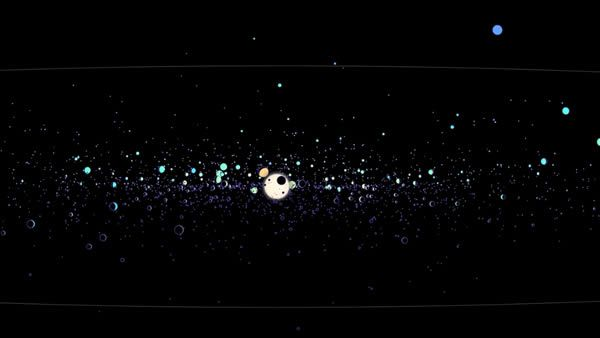
\includegraphics[width=0.8\textwidth]{images/worlds.jpg}
  \caption{Image of Worlds Visualisation}
\end{figure}

What does this provide me?

\subsection{The Kepler Orrery and The Kepler Orrery 2 - Non interactive}
This illustrates the exoplanet candidates in their own solar systems. The orbit radii are to scale with respect to each other and planet sizes are to scale with respect to each other, but orbits and planet sizes are different scales. The colors are in order of semi-major axis: two-planet systems (242 in all) have a yellow outer planet; 3-planet (85) green, 4-planet (25) light blue, 5-planet (8) dark blue, 6-planet (1, Kepler-11) purple. http://kepler.nasa.gov/multimedia/animations/?ImageID=219
\begin{figure}[h!]
  \centering
      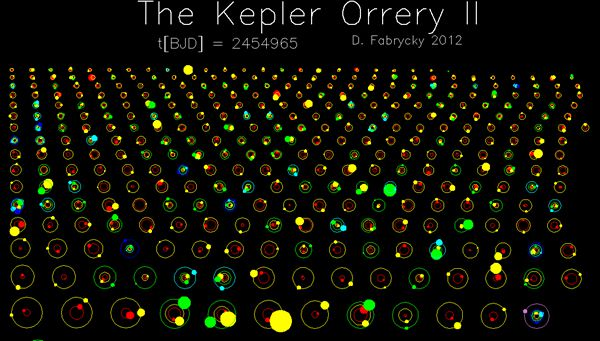
\includegraphics[width=0.8\textwidth]{images/orrery.jpg}
  \caption{Image of The Kepler Orrery Visualisation}
\end{figure}
This system exhibits small multiples, a grid of small similar graphics or charts, allowing them to be easily compared.
\\\\
What does this provide me?
\subsection{The Kepler Visualization Tool }
It displays all Kepler candidates, arranged as if orbiting a single star. Each candidate's estimated size, orbital speed, and orbital separation is accurately depicted, and each planet is color-coded according to its estimated effective temperature, with red being relatively hot and deep blue/violet being relatively cold. Mercury, Mars, Earth, and Jupiter are added for context. Two concentric rings plot distances of 0.5 and 1 astronomical units from the central star, and a pale blue line delineates Earth's location on two self-organizing charts. In the video posted above, the first chart in the sequence plots semi-major axis (i.e., average orbital separation) versus effective temperature, while the second plots semi-major axis versus planetary size.
\begin{figure}[h!]
  \centering
      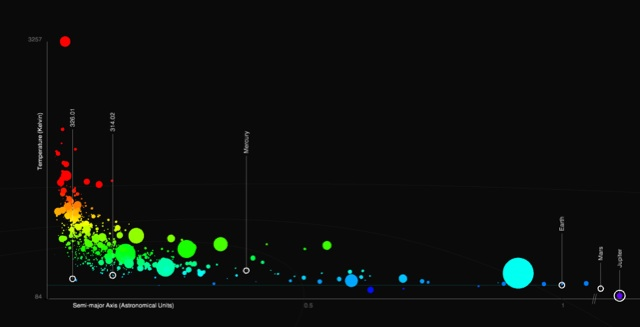
\includegraphics[width=0.8\textwidth]{images/kepler1.jpg}
  \caption{Image of The Kepler Orrery Visualisation}
\end{figure}
Important data trends emerge from this visualization. The abundance of smaller candidates and relative sparsity of larger ones clearly indicates that there are many tiny, meek worlds for every giant planet.
\\\\
What does this provide me?
\\\\
http://boingboing.net/2011/02/08/a-new-view-of-the-ga.html\\
http://kepler.nasa.gov/multimedia/animations/scienceconcepts/?ImageID=135
\subsection{Celestia - Interactive}
Celestia is a free real-time space simulation that lets you visually experience the universe in three dimensions
\\\\
Celestia is a computer program written in the computer language C++.  The code is Open Source, and may be examined and modified by anyone under the terms of the GNU Public License.
\\\\
\begin{figure}[h!]
  \centering
      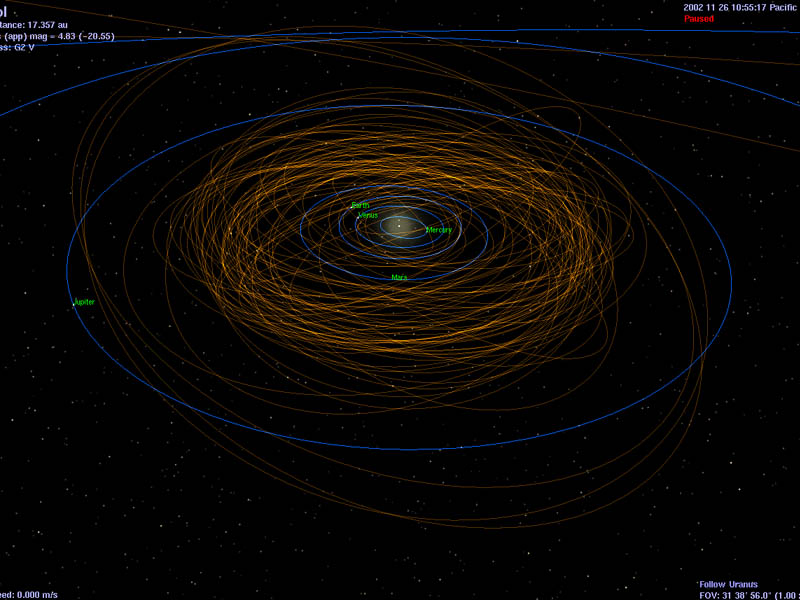
\includegraphics[width=0.8\textwidth]{images/celestia.jpg}
  \caption{Image of Celestia Visualisation}
\end{figure}
\\\\
http://www.shatters.net/celestia/
\\\\
What does this provide me?

\chapter{Technology and Design}
\section{Technology Option Exploration}
\subsection{Java using Swing or Processing}
Building a visualisation in Java would mean that I would be able to design it from the ground up. This would mean that there would be an almost non existent learning curve as I would not be extending an existing visualisation or learning a new tecchnology.  If I were to use the GUI library Swing, it would involve using a drawing canvas or another graphic rendering tool. However by using this solution over tailored and  proven visualization toolkits I would be limiting the quality of the system. This is because the built in drawing methods in Java are primitive compared to some of the visualisation libraries and frameworks available.
\\\\
A better option would be to use Processing. Processing is an open source programming language and development environment that was initially created to serve as a software sketchbook and to teach the fundamentals of computer programming with a visual context. Using processing would mean that the visualization could be built with Java while still using a successful visualisation framework. The most complete existing visualization using the same exoplanet dataset (Kepler Visualization Tool) is built using Processing . 
\\\\
Using this solution would involve learning the Processing language, however Processings is a library built in Java so the syntax is the same. This means the learning curve in in regards to the program itself should be shallow.
\\\\
Using processing and would mean that 3D elements could be included, this wouldn’t be possible with D3. However it does require a strong knowledge in 3D transformations which I do not possess. This may be a limiting factor in the speed at which I could understand the existing code and may push using this solution out of scope in favour of D3.
\\\\
IMAGE
\subsection{D3 (Data-Driven Documents)}
D3 is a JavaScript library that allows the displaying of data in dynamic graphics. Embedded within an HTML web page, the javascript D3.js library uses pre-built javascript functions to select elements, create Scalable Vector Graphic (SVG) objects, style them, and add transitions, dynamic effects and tooltips. Large datasets can be easily bound to SVG objects using simple D3 functions to generate rich charts and diagrams. D3 was created because of the need for a balance of expressiveness, efficiency, and accessibility that previous visualization toolkits did not allow \cite{d3}. 
\\\\
D3 allows the binding of input data to arbitrary input elements. This means that the exoplanet dataset can easily be bound to SVG elements for creating visualizations. D3 adopts the W3C Selectors API to identify document elements queried. This results in a rich but concise selection method of elements in a visualisation. 
\\\\
D3 allows debugging thanks to google chrome and other modern browsers development tools. A downside to D3 is that it does not allow 3D diagrams, although it does allow pseudo 3D by using the painter's algorithm and textures.
\\\\
\begin{figure}[h!]
  \centering
      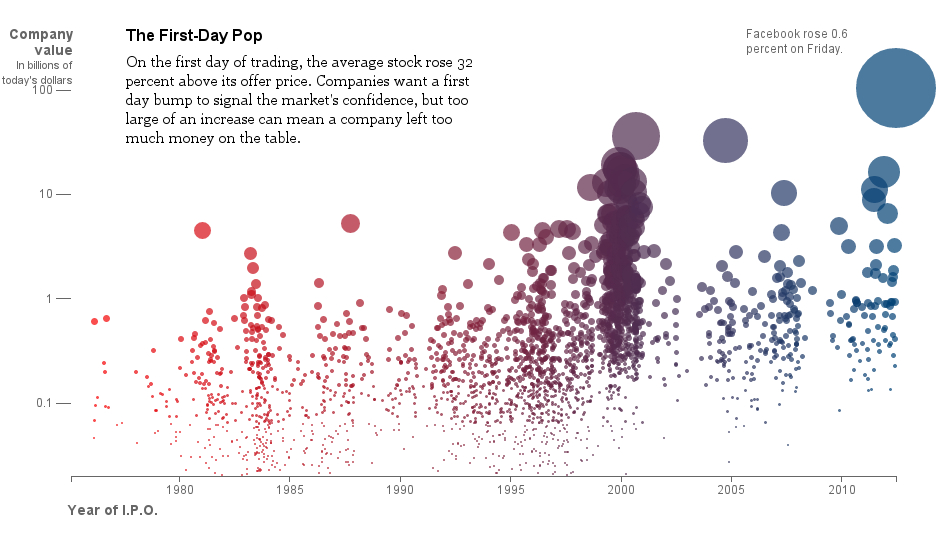
\includegraphics[width=0.8\textwidth]{images/d31.jpg}
  \caption{Example system in D3 showing Facebook statistics $http://www.nytimes.com/interactive/2012/05/17/business/dealbook/how-the-facebook-offering-compares.html$}
\end{figure}
\subsection{Prefuse}
Prefuse is a set of software tools for creating rich interactive data visualizations \cite{prefuse}. The Prefuse toolkit provides a visualization framework for Java.  It supports a set of features for visualizing and interacting with data. It provides optimized data structures for tables, graphs, and trees. It can be used to build standalone applications, visual components embedded in larger applications, and web applets. Prefuse to greatly simplifies the process of representing and efficiently handling data, mapping data to visual representations (e.g., through spatial position, size, shape, color, etc), and interacting with the data. 
\\\\
To use Prefuse a basic familiarity with the Java is required, including setting up and building Java projects. A knowledge of Swing or another similar user interface toolkit is also useful for understanding some of the concepts behind prefuse and for integrating prefuse visualizations into larger applications. Experience with database systems is also helpful.
\\\\
HOWEVER
\section{Design Decisions}
It needs to have a low learning curve as the time available to learn a technology is small
\\\\
3D is an advantage as it is more immersive(REF)
\\\\
It needs to be suited towards visualizations with prior evidence that it can produce quality visualisations.
\\\\
It needs to allow user interaction with dynamic transitions.
\\\\
It would be advantageous  if there is a pre existing solution with a similar dataset as it would mean that in depth design work would not be required.
\\\\
TODO
\section{Choosing My Solution}
TABLE INSERT
\\\\
The technology that was chosen for this project was Processing. This was because of the advantages it had over the other options is shown in the table above as well as having an existing solution with the Kepler dataset. It also has a shallow learning curve as it uses Java as the programming language. I also only need to learn the required code needed for Processing which the API and online examples make easy, as well as the opensource libraries available. The only apparent downside to the language is that to effectively use the 3D functionality it requires knowledge of 3D transformations. However this negative aspect is overcome by its other positive features and the fact that I can learn 3D transormations.
\\\\
As well as using Processing as the tool for the visualisation, I will also extend the existing Kepler Visualization Tool. This is because it provides a basis for a 3D visualisation as well as TODO.
\\\\
//TODO open source, further improved
\\\\
//TODO To mitigate the risk of inadequate knowledge of 3D transformations
\\\\
//TODO Because this solution has these advantages over the other solutions, and even though it does still have disadvantages. It has the highest chance of providing the best solution because 
\section{My Chosen Solution}
The existing system built with Processing is a simple visualisation focusing on displaying the candidate Exoplanets temperatures and their locations in relation to their distance from their nearest star, so that a sense of scale can be perceived. Each candidate’s estimated size, orbital speed, and orbital separation is accurately depicted, and each planet is color-coded according to its estimated effective temperature.
\\\\
By choosing to extend this existing solution the benefits of using Java and processing would be joined by the benefits of using an effective visualisation tool. \\
\begin{figure}[h!]
  \centering
      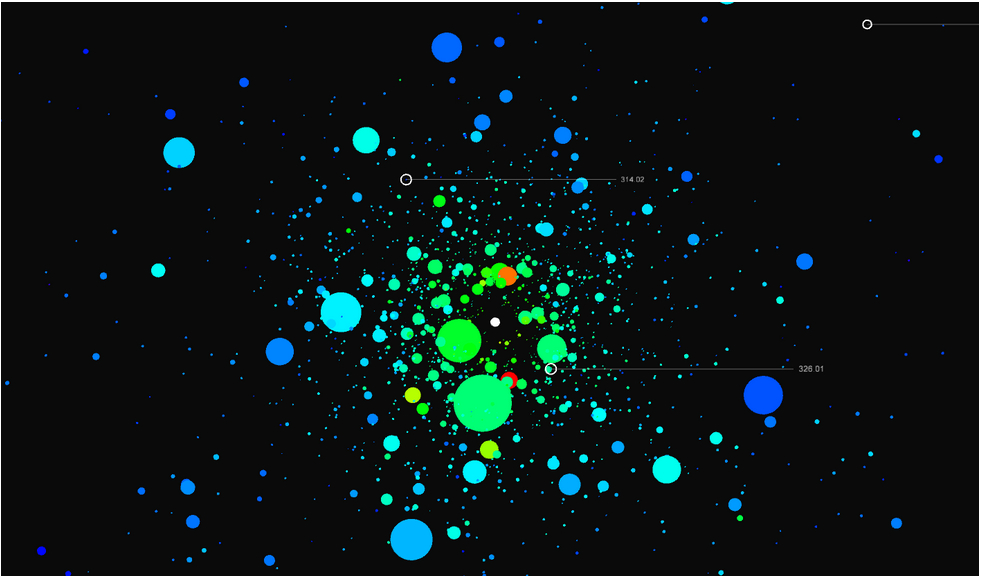
\includegraphics[width=0.8\textwidth]{images/kepler_orbital.jpg}
  \caption{Kepler Visualisation Tool Orbital View}
\end{figure}
\begin{figure}[h!]
  \centering
      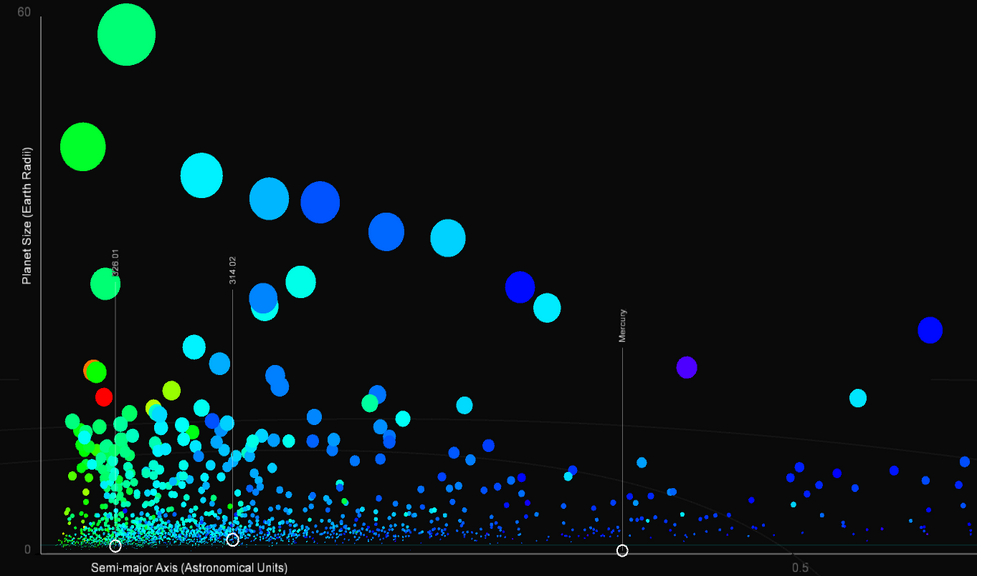
\includegraphics[width=0.8\textwidth]{images/kepler_graph.jpg}
  \caption{Kepler Visualisation Tool Graph View}
\end{figure}
The existing work in this system would serve as foundation for this project. TODO
\\\\
Because much of the visual aspects, and initial data manipulation of the existing system are already complete. It means that implementing the features needed for this projects completion could be focussed on more heavily and larger improvements to the existing system can be undertaken, such as better labeling and information displays and user interaction methods.
\section{Existing work on Kepler Visualization Tool}
INTODUCTION
\subsection{Existing Layouts}
The existing visualisation has 2 different layouts for the data
\\\\
1. Orbital Layout - Shows exoplanets orbiting a single stars (Figure 3.2)
\\\\
2. Graph Layout - Used to display planets on x,y scale using attributes (Figure 3.3)

\subsection{Existing Interaction Techniques}
The only interaction techniques in the existing system are:
\\\\
\begin{figure}[h!]
  \centering
      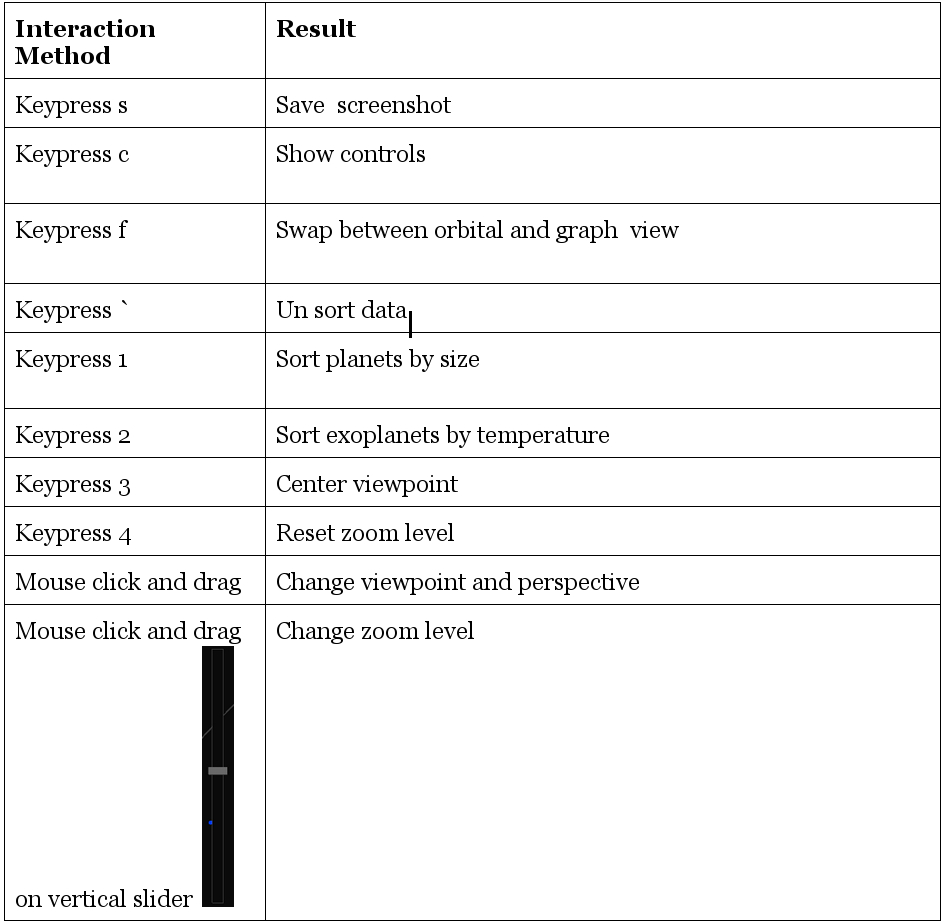
\includegraphics[width=0.8\textwidth]{images/table.jpg}
  \caption{Table of exisiting interaction methods in system}
\end{figure}
TODO\\
DISCUSS WHAT ELSE IS NEEDED AND WHY

\chapter{Visualisation Design}
\section{Required User Interactions}
There are a set of interaction methods that will be important for this visualization. These methods are:
\begin{enumerate}
 \item Select planets for further analysis
 \item Select planet attribute to sort by
 \item TODO
\end{enumerate}
There are also improvements needed for the existing system to improve user interaction. TODO why ?. These improvements are:
\begin{enumerate}
 \item A panel containing buttons for each of the views changes
 \item Include scroll to zoom functionality
\end{enumerate}
\section{Required Visual Elements}
TODO
\section{Layout Requirements}
By using abstract user interface design the layout and configuration of each element can be planned and coordinated without the need for excessive details which are likely to change throughout the course of the project (e.g., colours and content).
\\\\
The visualisation elements needed to convey the information in the dataset can be broken into 4 sections. This means that there should be a section in the layout of the visualization that corresponds to each. I have created 3 potential layouts and the optimal choice will be one that induces the lowest cognitive and load for users and is the most intuitive.  I am able to focus on creating a layout that does not create unneeded extraneous load [cognitive load citation] on users. Doing this means that each section of the visualization needs to be separated spatially from one another so that the cognition needed to visually separate each section is minimal.  
\\\\
For this visualisation there is the need for 4 user interface boxes. 
\begin{enumerate}
\item Main Panel: Display the main visualisation. The other panels will be used to support this panel.
 \item Interaction Panel: Display the interaction components for the visualisation. This is because the existing solution has only keypresses as the way of modifying the visualisation. This is not sufficient as there is no indication in the system of how to use these. Also the proposed extensions to the system will require more advanced user interaction elements
\item Selected Planet Panel: Display the information about a selected planet.
\item Comparison Panel: Display a comparison between 2 selected elements.
\end{enumerate}
IMAGE
\\\\
These layouts will need to be evaluated to discover which is the most effective. It is possible that none of these options are suitable and the layout may need to be redesigned, however as the functionality will be implemented, changing the layout will be a trivial matter. 

\section{User Interface Design}
$http://web.cs.wpi.edu/~matt/courses/cs563/talks/smartin/int_design.html$
\section{Screen Mockup: Visualisation Interaction Panel(Panel 1)}

\begin{figure}[h!]
  \centering
      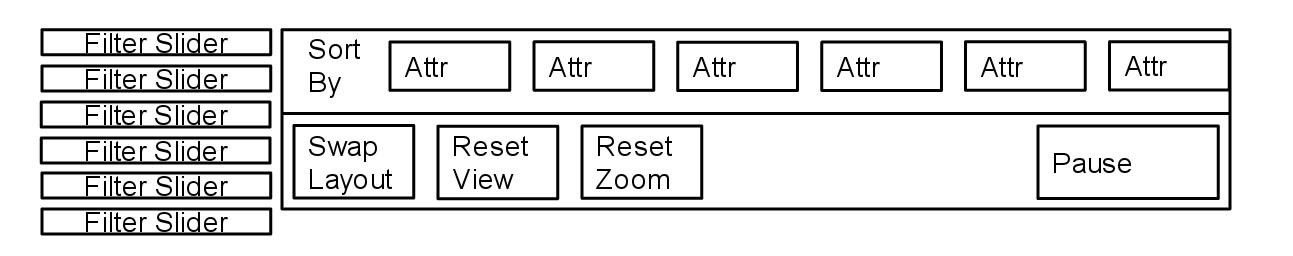
\includegraphics[width=0.8\textwidth]{images/interaction_mock.jpg}
  \caption{Mockup of interaction panel}
\end{figure}

By keeping the most widely used interaction elements at the edges of the visualisation it will allow mouse flicking for efficient component selection. Also by allowing GUI interactive elements as well as maintaining the existing key press interactivity it should allow a good balance between advanced and novice users. To improve this, each of the on screen interactive elements will also depict the keystroke that yields the same functionality as a way of transitioning novice users to advanced(REFERENCES)
\\\\
FITS LAY AND STEERING LAW
\section{Screen Mockup: Selected Planet Panel (Panel 2)}
\begin{figure}[H]
  \centering
      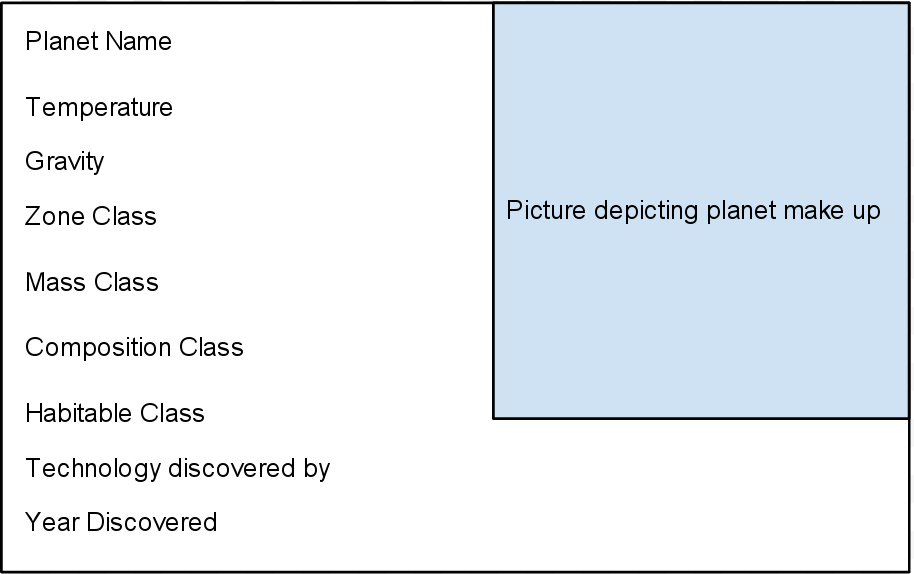
\includegraphics[width=0.8\textwidth]{images/planet_mock.jpg}
  \caption{Mockup of planet information panel}
\end{figure}

Explanation:
\\
Using the vertical placement of exo planets to display their ESI while maintaining their horizontal placement should aid in comprehension by users about the comparisons to Earth
\section{Screen Mockup: Comparison to Earth panel (Panel 3)}
\section{Screen Mockup: Main panel (Panel 4)}
\subsection{Earth Similarity Index (ESIs, ESIi, ESIg) }
\begin{figure}[H]
  \centering
      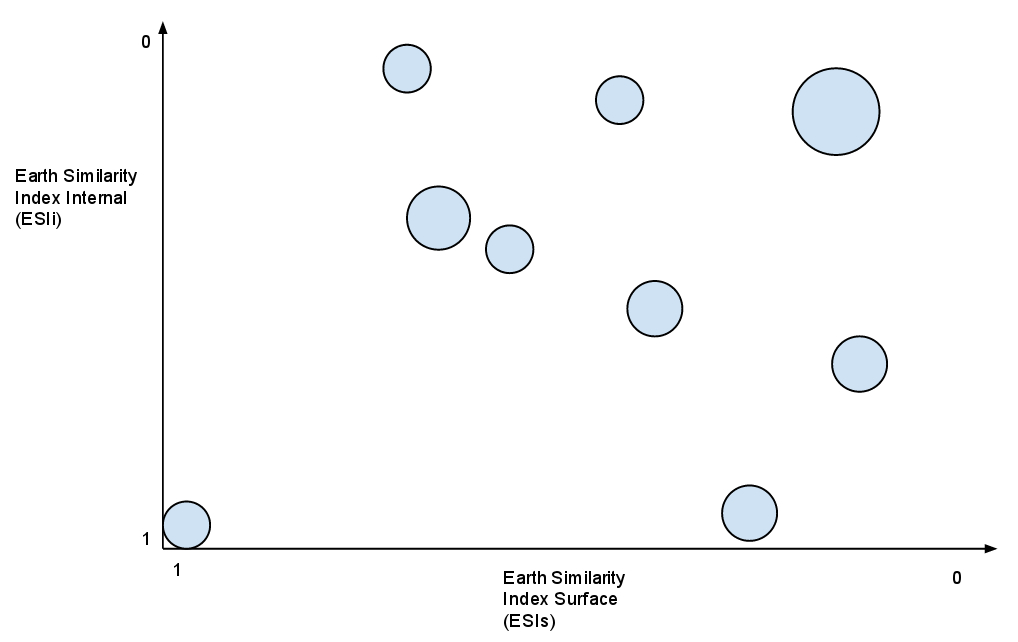
\includegraphics[width=0.8\textwidth]{images/esi_mock.jpg}
  \caption{Mockup of planet ESI view in graph layout}
\end{figure}
Explanation:\\
Using the vertical placement of exo planets to display their ESI while maintaining their horizontal placement should aid in comprehension by users about the comparisons to Earth
\\\\
Placement:\\
Exoplanets\\
Vertical Alignment = ESIg\\
Horizontal Alignment = Semi-Major-Axis(AU)
\\\\
Earth\\
Vertical Alignment = 1.0 ESIg\\
Horizontal Alignment = Center of exoplanet orbit
\\\\
Star\\
Vertical Alignment = 0.0 ESIg\\
Horizontal Alignment =  Center of exoplanet orbit

\chapter{Progress}

\section{Progress Made}
I have implemented 
\section{Difficulties encountered with implementation}
Problem:\\
The existing solution was implemented in a way that only the z axis location of each exoplanet could be modified. This meant that to display multivariate data on more than one axis the method of translating planets needed to be modified.
\\\\
Solution:\\
I extended the existing draw method of planets where the x and y locations of exoplanets were set so that it can be changed. However there is still a problem that it does not animate this change, this will require modifying the method further to incrementally move the planets when the axis are modified.
\\\\
Problem:\\
Any on screen gui elements were placed inside the visualisation on the same plane as the planets, and so are zoomable as well as rotatable instead of being fixed as is needed for a GUI
\\\\
Solution:\\
I currently have a partial solution which is to use multiple frames for each window component. However this is not optimal as the main window needs to be selected for key presses to work even though it does allow the user to rearrange the different windows as they wish. 
\\\\
Problem: \\
Due to the large number of items to be displayed on screen there is a large amount of performance loss and sometimes crashes the visualisation due to an out of memory exception or simply freezing.
\\\\
Solution:\\
Filtering of data to reduce the amount of planets being rendered reduces this problem but does not solve it. This is still an outstanding issue.
\\\\
Problem:\\
When filtering the exoplanets there is a lag in the rendering. 
\\\\
Solution:\\
I will find a more efficient way of sorting and filtering data. This is still an outstanding issue.
\\\\
Problem:\\
When a planet is selected and a button is clicked a NullPointerException is thrown
\\\\
Solution:\\
It was because the core planets of our solar system were being checked against due to them being considered feature planets when they should have been excluded. I refactored it so that they are now corePlanets and so the feature boolean can be used safely.
\chapter{Future Plans}
\section{Implementation}
\section{Evaluation}
The evaluation of this system will be based on a user study of the final visualisation design
chosen and implemented. The user study will need to be designed to evaluate whether this
system can effectively display the answers to the questions introduced previously and maintain
user interest. The evaluation would also focus on the users ability to efficiently navigate
through the 3D structure, and to accurately and precisely select exoplanets for further study,
and accurately and precisely manipulate filtering tools.The evaluation will be based on both
qualitative and quantitative analysis of users interaction with the system.
The evaluation will have 20 subjects, for a 10 minute evaluation. This timeframe is similar to
the amount of time that someone would spend at an information terminal in an observatory.
During the evaluation the users will be monitored either in person or by camera to evaluate
their experiences with the system.
\section{Report}
\chapter{Conclusion}
%%%%%%%%%%%%%%%%%%%%%%%%%%%%%%%%%%%%%%%%%%%%%%%%%%%%%%%
\backmatter
%%%%%%%%%%%%%%%%%%%%%%%%%%%%%%%%%%%%%%%%%%%%%%%%%%%%%%%


%\bibliographystyle{ieeetr}
\nocite{*}
\bibliographystyle{acm}
\bibliography{sample}


\end{document}
